\textbf{\underline{OZ 1 - Herhaling - Oefening 4:}}
\vspace{0.5cm}


\begin{minipage}{.73\textwidth}
    Protonen worden met een snelheid $v_i = 9, 55 \text{km/s}$ in een regio
    met een uniform elektrische veld $\Vec{E} = -720\hat{k} \text{N/C}$ geschoten (zie figuur). Het is de bedoeling dat de protonenstraal een doelwit raakt dat zich $R = 1, 27 $ mm van het punt bevindt waar de
    straal het elektrisch veld binnenkomt. Bereken onder welke twee hoeken $\theta$ de protonenstraal het
    doelwit raakt en hoe lang de protonen zich boven het vlak in de tekening bevinden. (Verwaarloos
    de zwaartekracht, de massa van een proton is immers $1, 67E-27 $ kg).
\end{minipage}
\begin{minipage}{.23\textwidth}
    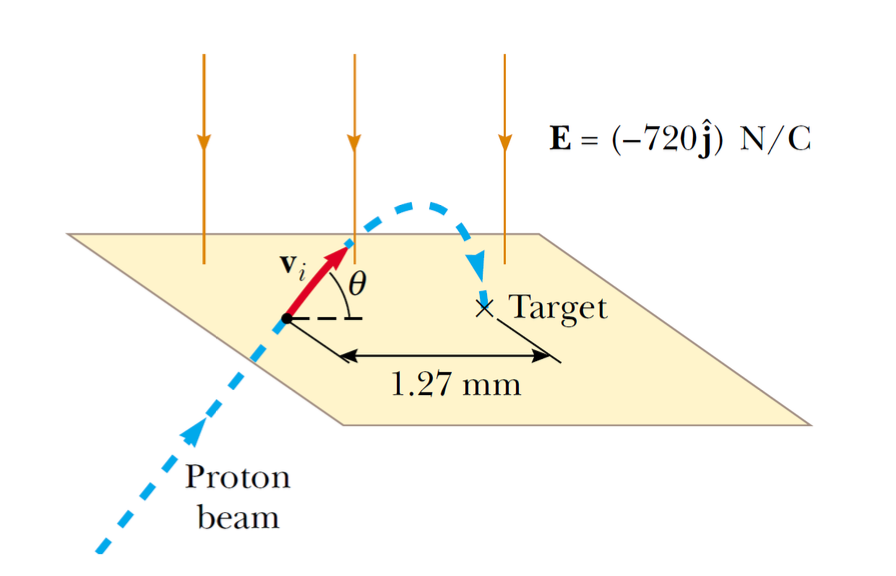
\includegraphics[scale = 0.31]{oz01/herhaling/resources/ElektronenElektrischVeld.png}
\end{minipage}

% \begin{description}[labelwidth=1.5cm, leftmargin=!]
%     \item[Geg. :]  
%     \item[Gevr. :]  
%     \item[Opl. :]   
% \end{description}

\begin{description}[labelwidth=1.5cm, leftmargin=!]
    \item[Geg. :]   $v_i = 9, 55 \text{km/s}$, $\Vec{E} = -720\hat{k} \text{N/C}$, $R = 1, 27 $ mm, $m_p = 1, 67E-27$ kg, $q = q_p$
    \item[Gevr. :]  $\theta$ ?
    \item[Opl. :]  
    \item[]
        \vspace{-0.7cm}
        \begin{minipage}{0.65\textwidth}
            Een lading in een elektrisch veld ondervindt een elektrische kracht, namelijk
            \begin{equation*}
                \Vec{F}_e = q_p\Vec{E}
            \end{equation*}
            waarbij parallel aan het veld is. We vinden door de tweede wet van Newton dat
            \begin{equation*}
                \Vec{a} = \frac{q_p}{m_p}\Vec{E}
            \end{equation*}
            waardoor deze oefening trivialiseert tot een projectielbeweging oefening. Neem het punt waar de protonen doorvliegen als de oorsprong.
        \end{minipage}
        \hspace{0.5cm}\begin{minipage}{.31\textwidth}
            \begin{center}
                \def\arraystretch{2}
                \begin{tabular}{c|c|c}
                     & $x$ & $y$ \\ \hline
                     $ r $ & $  v_i\cos(\theta)t $ & $  v_i\sin(\theta) - \frac{at^2}{2} $ \\ \hline
                     $ v $ & $ v_i\cos(\theta) $ & $ v_i\sin(\theta) - at $  \\ \hline
                     $ a $ & $ 0 $ & $ -a $ 
                \end{tabular}
            \end{center}
        \end{minipage}
    
        Stel $v_y$ de verticale snelheid op het hoogste punt, dan
        \begin{equation*}
            \frac{v_y-v_{0,y}}{a_y} = t
        \end{equation*}
        ofwel
        \begin{equation*}
            \frac{2v_i\sin(\theta)}{a_y} = t
        \end{equation*}
        waarbij we maal twee doen om een vergelijking te hebben voor heel de beweging, want het maxima komt voor in het midden van de beweging. We weten voor de x-as dat
        \begin{align*}
            R_x 
                &= v_i\cos(\theta)t \\
                &= v_i\cos(\theta)\left( \frac{2v_i\sin(\theta)}{a_y}\right) \\
                &=  \frac{v_i^2}{a_y} \sin(2\theta)
        \end{align*}
        wat we kunnen herwerken tot $\theta$
        \begin{equation*}
            \theta = \frac{1}{2}\sin^{-1}\left(\frac{v_i^2}{a_y} \sin(2\theta)\right) = 36.9^{\circ} \ \text{en} \ 53.1^{\circ} 
        \end{equation*}
        wat we kunnen invullen in de verticale snelheidsvergelijking om de volgende tijden te krijgen
        \begin{equation*}
            t_{36.9^{\circ}} = 1.66 \cdot 10^{-7} \text{s} \ \text{en} \ t_{53.1^{\circ}} = 2.21 \cdot 10^{-7} \text{s}
        \end{equation*}
        
    
\end{description}
